\chapter{Dimensionnement \& Choix du matériel}

\section{Système de motorisation}

\subsection{Choix du moteur}

\subsubsection{Modes de fonctionnement}

Le moteur constitue l'actionneur central du banc de test. Il doit répondre aux exigences de deux modes de fonctionnement distincts :

\begin{itemize}
    \item \textbf{Mode vieillissement accéléré~:} le moteur effectue des impulsions de rotation répétées, chacune inférieure à 2 tours, afin de simuler le remontage manuel d'une montre. Ces impulsions sont réalisées à une vitesse de 350 tours/min avec une accélération pouvant atteindre 5000 tours/min², ce qui impose au moteur des démarrages et arrêts dynamiques fréquents.

    \item \textbf{Mode réserve de marche~:} ce mode se déroule en deux phases. Dans un premier temps, le moteur entraîne la tige du mouvement à 50 tours/min pour remonter le barillet complètement puis le dévider du nombre de tours souhaité. Dans un second temps, le moteur se maintient en position bloquée pendant environ 24 heures, empêchant toute rotation du système pendant que la caméra enregistre le déroulement du barillet.
\end{itemize}

\subsubsection{Justification du choix : moteur pas à pas}

Un moteur pas à pas a été retenu. Ce choix se justifie par trois critères majeurs :

\begin{itemize}
    \setlength{\itemsep}{6pt}
    \item \textbf{Contrôle précis de la position angulaire~:} Le nombre de tours doit être connu avec précision. En considérant une résolution minimale requise de 0,02 tour (soit 7,2°), un moteur pas à pas standard à 200 pas/tour offre un pas de 1,8°, soit une résolution quatre fois supérieure à l'exigence.
    
    \item \textbf{Maintien statique sans asservissement~:} En mode réserve de marche, la phase de blocage sur 24 heures ne nécessite aucun encodeur ni boucle de retour~; le moteur pas à pas maintient naturellement sa position dès lors qu'il est alimenté, ce qu'aucun moteur à courant continu ne peut garantir sans frein ou asservissement supplémentaire.
    
    \item \textbf{Commande simple et reproductible~:} Le nombre de pas envoyés détermine directement l'angle parcouru, sans calibration préalable.
\end{itemize}

\subsubsection{Sélection du format et du modèle}

Parmi les formats normalisés de moteurs pas à pas à 200 pas/tour (NEMA 8, NEMA 11, NEMA 17), le format NEMA 11 a été retenu pour optimiser la compacité.

D'après les données techniques fournies, le couple maximal que le barillet peut exercer est de 10,2 mN·m. Compte tenu d'un rapport de réduction de 3,33 entre la tige et le barillet, le couple que le moteur doit exercer pour remonter le mouvement est de 3,24 mN·m. En appliquant une marge de sécurité pour les frottements mécaniques et les variations de charge, le couple minimal requis est fixé à :

\begin{equation}
    C_{\text{requis}} = 4 \text{ mN·m}
    \label{eq:couple_requis}
\end{equation}

\noindent où $C_{\text{requis}}$ est le couple minimal requis pour maintenir le système et éviter qu'il se décharge spontanément sous l'effet du ressort.

\vspace{0.3cm}

Pour le calcul du couple dynamique, le moment d'inertie de la fourche est estimé à 8,67 g·cm² d'après les mesures SolidWorks~; le système complet est estimé à environ 15 g·cm². Le couple dynamique requis pour les accélérations est donc :

\begin{equation}
    C_{\text{dynamique}} = J_{\text{système}} \times \alpha = 15 \times 5000 \approx 0,02 \text{ mN·m}
    \label{eq:couple_dynamique}
\end{equation}

\noindent où $J_{\text{système}} = 15$ g·cm² (moment d'inertie du système complet) et $\alpha = 5000$ tours/min² (accélération maximale). Cette valeur est négligeable au vu de son ordre de grandeur.

\vspace{0.3cm}

Le moteur retenu est le \textbf{NEMA11-01} de Joy-IT (référence 28SHD4201-20) \cite{moons_nema11, joytechnik_nema11_01}. Ses caractéristiques principales sont présentées au tableau~\ref{tab:specs_moteur}:

\begin{table}[H]
  \centering
  \caption{Caractéristiques du moteur pas à pas NEMA11-01}
  \label{tab:specs_moteur}
  \begin{tabular}{ll}
    \toprule
    \textbf{Paramètre} & \textbf{Valeur} \\
    \midrule
    Couple de maintien & 55 mN·m \\
    Couple de détente & 5 mN·m \\
    Courant nominal & 0,42 A \\
    Tension nominale & 5,0 V \\
    Angle de pas & 1,8° $\pm$ 5\% \\
    Résistance de phase & 11,9 Ω \\
    Inductance de phase & 7,8 mH \\
    \bottomrule
  \end{tabular}
\end{table}

\vspace{0.3cm}

La courbe couple-vitesse a été établie en se référant aux données du fabricant MOONS', dont les moteurs présentent des spécifications électriques et mécaniques similaires au NEMA11-01.

\begin{figure}[H]
    \centering
    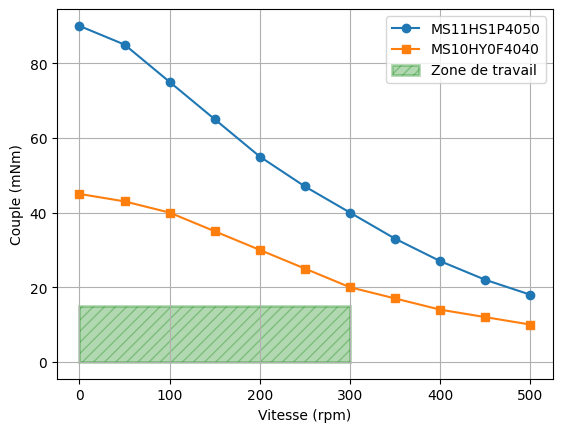
\includegraphics[width=1\textwidth]{assets/figures/Dimensionement/graphe courbe couple vitesse moteur.png}
    \caption{Courbes couple-vitesse des moteurs NEMA}
    \label{fig:couple_vitesse}
\end{figure}

\newpage

\subsection{Choix du driver}

\subsubsection{Critères de sélection}

Le driver doit satisfaire trois critères~: la compatibilité mécanique avec le moteur, une plage de courant adaptée à la précision requise, et la capacité à piloter plusieurs axes depuis un ordinateur.

\subsubsection{Compatibilité mécanique et plage de courant}

Le moteur NEMA 11 a des dimensions de 28 x 28 mm. Le driver doit être montable directement à l'arrière d'un tel moteur. Le courant nominal du moteur est de 0,42 A, donc un driver avec une plage de courant basse offrant une meilleure précision de limitation du couple est souhaité.

Avec 32 niveaux de courant (0 à 31), l'échelon de courant minimal vaut :

\begin{equation}
    \Delta I = \frac{I_{\text{max}}}{31} = \frac{0,7}{31} \approx 22,6 \text{ mA}
    \label{eq:echelon_courant}
\end{equation}

\noindent où $I_{\text{max}} = 0,7$ A (courant maximal du driver) et 31 est le nombre d'incréments disponibles.

\vspace{0.3cm}

Le nombre de niveaux utiles jusqu'au courant nominal du moteur est :

\begin{equation}
    N_{\text{utiles}} = \left\lfloor \frac{I_{\text{nom}}}{\Delta I} \right\rfloor = \left\lfloor \frac{0,42}{0,0226} \right\rfloor \approx 18 \text{ niveaux}
    \label{eq:niveaux_utiles}
\end{equation}

\noindent où $I_{\text{nom}} = 0,42$ A (courant nominal du moteur).

\vspace{0.3cm}

En tenant compte du couple de maintien du moteur, la précision de limitation du couple est :

\begin{equation}
    \Delta C = \frac{C_{\text{maintien}}}{N_{\text{utiles}}} = \frac{55}{18} \approx 3 \text{ mN·m}
    \label{eq:precision_couple}
\end{equation}

\noindent où $C_{\text{maintien}} = 55$ mN·m (couple de maintien du moteur) et $N_{\text{utiles}} = 18$ niveaux. Cette précision de $\pm 3$ mN·m est suffisante pour l'application visée.

\subsubsection{Driver sélectionné : TMCM-1021}

Le \textbf{TMCM-1021} a été retenu. Ses caractéristiques principales sont présentées au tableau~\ref{tab:specs_driver}:

\begin{table}[H]
  \centering
  \caption{Caractéristiques du driver TMCM-1021}
  \label{tab:specs_driver}
  \begin{tabular}{ll}
    \toprule
    \textbf{Paramètre} & \textbf{Valeur} \\
    \midrule
    Format & 28 x 28 mm (NEMA 11) \\
    Plage de courant basse & 0,7 A RMS (programmable) \\
    Tension d'alimentation & 9 à 28 V \\
    Interface de communication & RS485 (protocole TMCL) \\
    Capteur intégré & SensOstep (encodeur magnétique) \\
    Fonctionnalités avancées & stallGuard2, coolStep, stealthChop \\
    \bottomrule
  \end{tabular}
\end{table}

\subsubsection{Avantages du TMCM-1021}

\begin{itemize}
    \item \textbf{Pilotage multi-axes~:} Le bus RS485 permet de connecter jusqu'à 255 modules sur un seul câble. Chaque driver se voit attribuer une adresse unique, permettant au script Python de les commander indépendamment via un simple adaptateur USB/RS485. Cette architecture est adaptée à une évolution vers un système multi-axes.
    
    \item \textbf{Interface série~:} Le TMCM-1021 peut être contrôlé directement depuis un script Python sans microcontrôleur intermédiaire. Le fabricant Trinamic (ADI) propose une gamme intégrant le contrôleur, le driver et la communication, programmables via le langage TMCL et la bibliothèque Python PyTrinamic~\cite{trinamic_pytrinamic}.
\end{itemize}

\newpage

\subsection{Alimentation du moteur}

L'alimentation du moteur est assurée par le bloc secteur \textbf{RS-25-24} (Mean Well).

\subsubsection{Caractéristiques de l'alimentation}

\begin{itemize}
    \item Tension de sortie : $V_{\text{alim}} = 24$ V DC
    \item Courant maximal : $I_{\text{max}} = 1,1$ A
\end{itemize}

\subsubsection{Vérification de la compatibilité}

La puissance disponible est :

\begin{equation}
    P_{\text{alim}} = V_{\text{alim}} \times I_{\text{max}} = 24 \times 1,1 = 26,4 \text{ W}
    \label{eq:puissance_alim}
\end{equation}

\noindent où $V_{\text{alim}} = 24$ V (tension de sortie) et $I_{\text{max}} = 1,1$ A (courant maximal disponible).

\vspace{0.3cm}

La puissance consommée par le moteur en fonctionnement nominal est :

\begin{equation}
    P_{\text{moteur}} = V_{\text{moteur}} \times I_{\text{moteur}} = 24 \times 0,42 = 10,1 \text{ W}
    \label{eq:puissance_moteur}
\end{equation}

\noindent où $V_{\text{moteur}} = 24$ V (tension moteur) et $I_{\text{moteur}} = 0,42$ A (courant nominal du moteur).

\vspace{0.3cm}

L'alimentation fournit donc une marge de sécurité de :

\begin{equation}
    \text{Marge} = \frac{P_{\text{alim}} - P_{\text{moteur}}}{P_{\text{alim}}} \times 100\% = \frac{26,4 - 10,1}{26,4} \times 100\% \approx 62\%
    \label{eq:marge_puissance}
\end{equation}

Cette marge permet d'accommoder des pics de consommation ou l'ajout de composants futurs.

\newpage

\section{Système d'acquisition optique}

\subsection{Choix de la caméra}

\subsubsection{Dimensionnement et calcul de résolution}

La caméra doit assurer une détection fiable du fonctionnement du mouvement de montre. Pour ce faire, l'élément le plus fin à détecter est la largeur de l'aiguille des secondes, estimée à 0,15 mm. Pour garantir une détection fiable par traitement d'image, au moins 5 pixels doivent couvrir cette dimension.

La résolution requise est donc :

\begin{equation}
    R_{\text{requise}} = \frac{d_{\text{min}}}{N_{\text{pixels}}} = \frac{0,15}{5} = 0,030 \text{ mm/pixel}
    \label{eq:resolution_spatiale}
\end{equation}

\noindent où $d_{\text{min}}$ est la largeur minimale à détecter en $[mm]$ et $N_{\text{pixels}}$ est le nombre minimal de pixels requis sur cette distance.

\vspace{0.3cm}

Cela correspond à environ \textbf{33 pixels/mm}. Le mouvement de montre le plus grand à observer fait $30$ mm de diamètre. On souhaite que la zone observée par la caméra soit légèrement plus large, soit $40 \times 40$ mm. Le nombre minimal de pixels du capteur en horizontal est donc :

\begin{equation}
    N_{\text{capteur}} = \frac{\text{Zone de travail}}{R_{\text{requise}}} = \frac{40}{0,030} \approx 1333 \text{ pixels}
    \label{eq:resolution_capteur}
\end{equation}

\noindent où Zone de travail = 40 mm (dimension du champ inspecté) et $R_{\text{requise}} = 0,030$ mm/pixel (résolution spatiale requise).

\subsubsection{Caméra sélectionnée}

Le modèle retenu est le \textbf{VEN-505-36U3C-M01} \cite{va_imaging_ven505}, équipé d'un capteur Sony IMX335 de format 1/2,8". Cette résolution de 2592 x 1944 pixels (5 MP) dépasse largement l'exigence minimale de 1333 pixels, offrant une excellente marge de confort. Ses caractéristiques principales sont présentées au tableau~\ref{tab:specs_camera}:

\begin{table}[H]
  \centering
  \caption{Caractéristiques de la caméra VEN-505-36U3C-M01}
  \label{tab:specs_camera}
  \begin{tabular}{ll}
    \toprule
    \textbf{Paramètre} & \textbf{Valeur} \\
    \midrule
    Capteur & Sony IMX335 \\
    Format du capteur & 1/2,8" \\
    Résolution & 2592 x 1944 pixels (5 MP) \\
    Largeur du capteur & 5,37 mm \\
    Hauteur du capteur & 4,04 mm \\
    Interface & USB 3.0 \\
    Connecteur caméra & C-mount \\
    \bottomrule
  \end{tabular}
\end{table} 

\subsection{Choix de l'objectif}

\subsubsection{Dimensionnement de l'objectif}

La zone d'inspection souhaitée est un champ de $40 \times 40$ mm. Le grandissement optique nécessaire est déterminé par la dimension limitante (largeur du capteur par rapport à la largeur du champ) :

\begin{equation}
    m = \frac{W_{\text{capteur}}}{\text{Champ d'inspection}} = \frac{5,37}{40} = 0,134
    \label{eq:grandissement}
\end{equation}

\noindent où $W_{\text{capteur}} = 5,37$ mm (largeur du capteur) et Champ d'inspection = 40 mm.

\vspace{0.3cm}

La distance de travail est fixée à \textbf{WD = 300 mm} pour permettre un montage pratique du système de motorisation et d'éclairage. À partir du grandissement calculé et de cette distance de travail, la focale requise de l'objectif est déterminée par la relation de conjugaison pour un objectif à focale fixe :

\begin{equation}
    f = \frac{WD}{1 + \frac{1}{m}} = \frac{300}{1 + \frac{1}{0,134}} = \frac{300}{8,46} \approx 35,5 \text{ mm}
    \label{eq:focale}
\end{equation}

\noindent où WD = 300 mm (distance de travail) et $m = 0,134$ (grandissement).

\vspace{0.3cm}

Une focale de 35 mm est donc requise pour satisfaire ces contraintes.

\subsubsection{Objectif sélectionné}

L'objectif retenu est le \textbf{VA-LCM-5MP-35MM-F1.4-015} \cite{va_imaging_lcm5mp}. Ses caractéristiques principales sont présentées au tableau~\ref{tab:specs_objectif}:

\begin{table}[H]
  \centering
  \caption{Caractéristiques de l'objectif VA-LCM-5MP-35MM-F1.4-015}
  \label{tab:specs_objectif}
  \begin{tabular}{ll}
    \toprule
    \textbf{Paramètre} & \textbf{Valeur} \\
    \midrule
    Focale fixe & 35 mm \\
    Ouverture & F/1.4 \\
    Monture & C-mount \\
    Optimisation & Capteurs format 2/3" et 1/2,8" \\
    Distance de travail & 300 mm \\
    \bottomrule
  \end{tabular}
\end{table}


\subsection{Système d'éclairage}

\subsubsection{Justification du choix d'une ring light}

L'observation du mouvement de montre en fonctionnement requiert un éclairage homogène et sans ombres. La ring light, montée coaxialement à l'objectif, fournit un éclairage diffus et uniforme du champ observé. À une distance de travail de 300 mm, un diamètre interne de 70 mm est requis pour ne pas obstruer le champ de vue de $40 \times 40$ mm. Un angle d'émission de 90° (horizontal) produit un éclairage rasant favorable à la mise en évidence des reliefs du mouvement.

\subsubsection{Ring light sélectionnée}

La ring light sélectionnée est le modèle \textbf{VA-RL3-70-90W} \cite{va_imaging_rl3}. Ses caractéristiques principales sont présentées au tableau~\ref{tab:specs_ringlight}:

\begin{table}[H]
  \centering
  \caption{Caractéristiques de la ring light VA-RL3-70-90W}
  \label{tab:specs_ringlight}
  \begin{tabular}{ll}
    \toprule
    \textbf{Paramètre} & \textbf{Valeur} \\
    \midrule
    Diamètre interne & 70 mm \\
    Angle d'émission des LEDs & 90° (émission horizontale) \\
    Puissance & 90 W \\
    Type d'éclairage & Éclairage rasant \\
    Montage & Coaxial à l'objectif \\
    \bottomrule
  \end{tabular}
\end{table}

\subsubsection{Contrôleur d'éclairage}

Le contrôleur retenu est le \textbf{VA-PS2-A4-60W-24V} \cite{va_imaging_ps2}. Ses caractéristiques principales sont présentées au tableau~\ref{tab:specs_controller}:

\begin{table}[H]
  \centering
  \caption{Caractéristiques du contrôleur VA-PS2-A4-60W-24V}
  \label{tab:specs_controller}
  \begin{tabular}{ll}
    \toprule
    \textbf{Paramètre} & \textbf{Valeur} \\
    \midrule
    Nombre de canaux & 4 canaux indépendants \\
    Tension d'alimentation & 24 V \\
    Puissance maximale & 60 W \\
    Réglage d'intensité & Gradateur intégré \\
    Entrée trigger & Oui \\
    Canaux utilisés dans ce projet & 1 canal \\
    \bottomrule
  \end{tabular}
\end{table}

\subsubsection{Filtration polarisante}

Les composants du mouvement de montre étant en métal poli, leur surface est fortement réfléchissante (réflexion spéculaire). Afin d'éliminer les reflets parasites et améliorer le contraste, une configuration en \textbf{polarisation croisée} est mise en place. 

Ce montage bloque la lumière directement réfléchie (composante spéculaire) et ne laisse passer que la composante diffuse, améliorant significativement le contraste de l'image. Cette configuration réduit le flux lumineux d'environ 20\%, ce qui est compensé par la puissance de la ring light (90 W).

Les composants optiques de filtration sélectionnés sont présentés au tableau~\ref{tab:specs_filters}:

\begin{table}[H]
  \centering
  \caption{Composants de filtration polarisante}
  \label{tab:specs_filters}
  \begin{tabular}{lll}
    \toprule
    \textbf{Composant} & \textbf{Référence} & \textbf{Fonction} \\
    \midrule
    Feuille polarisante & VA-LFT-LPOL-300x200 \cite{va_imaging_lft_sheet} & Devant ring light \\
    Filtre polarisant & VA-LFT-LPOL-M35.5 \cite{va_imaging_lft_lens} & Sur objectif (90°) \\
    \bottomrule
  \end{tabular}
\end{table}

\vspace{0.3cm}

\textbf{Résumé de l'acquisition~:} Le système optique offre une résolution de 15,4 $\mu$m/pixel sur un champ de 40 x 40 mm, avec une distance de travail de 300 mm et un éclairage rasant homogène. Ces caractéristiques permettent une détection fiable et reproductible des éventuels défauts du mouvement.
